
% -----------------------------------------------------------------------------------------------------------------
%\newpage
%\thispagestyle{empty}
%\rule{\linewidth}{2pt}
\chapter{Sistemas de ecuaciones no lineales}\label{capitulosistemas}

\section{Nueva familia de métodos de orden cuatro}\label{seccionlichensistemas}

Iniciamos este capítulo retomando la familia de métodos iterativos de orden 4, introducida en la Sección \ref{seccionlichen}, para resolver sistemas no lineales $F(x)=0$, probando su orden de convergencia local y aplicándola a la resolución numérica de la ecuación de Burgers (ya mencionada en el anterior capítulo). Recordemos que su expresión iterativa es

\begin{eqnarray}\label{s1}
y^{(k)} &=& x^{(k)} - \frac{2}{3}[F'(x^{(k)})]^{-1}F(x^{(k)}),\nonumber\\
x^{(k + 1)}& =& x^{(k)} - \left(I - \frac{3}{4}A^{-1}
B\right)[F'(x^{(k)})]^{-1}F(x^{(k)}),
\end{eqnarray}
donde $u ^{(k)} = [F'(x^{(k)})]^{-1}\left(F'(y^{(k)}) -
F'(x^{(k)})\right)$, $A= I + (\frac{3}{2} + \beta )u^{(k)}$,
$B=u^{(k)} + \beta u^{(k)^2}$ y $\beta$ es un parámetro arbitrario.

\subsection{Orden de convergencia}
\begin{theorem}
	Sea\ $\alpha\in D$  el cero de una función suficientemente diferenciable $F:D \in \mathbb{R}^n \rightarrow \mathbb{R}^n$, $n\geq 1$,
	en un conjunto convexo $D$ con una matriz Jacobiana no singular $F'(x)$ en $\alpha$, y sea también $x^{(0)}$ una aproximación inicial lo suficientemente cerca de la raiz $\alpha$.
	Para cualquier valor real del parámetro $\beta$, el esquema definido en
	(\ref{s1}) tiene orden de convergencia cuatro, y cuya ecuación del error está dada por
	\begin{equation*}%\label{2}
	e^{(k + 1)} = \left( \left(1 - \frac{8}{3}\beta\right)I  - {C_3}{C_2} +
	\frac{1}{9}{C_4}\right) e^{(k)^4} + O(e^{(k)^5}),
	\end{equation*}
	donde $C_j = \frac{1}{j!}[F'(\alpha )]^{ - 1}F^{(j)}(\alpha )$, $j =
	2,3,\ldots$ y ${e^{(k)}} = x^{(k)} - \alpha$.
\end{theorem}

\begin{proof}
	Si usamos el desarrollo en series de Taylor de $F\left(x^{(k)}\right)$ y $F'\left(x^{(k)}\right)$ alrededor de $\alpha$, obtenemos
	\begin{equation*}%\label{3}
	F({x^{(k)}}) = {F'}(\alpha )({e^{(k)}} + {C_2}{e^{(k)}}^2 +
	{C_3}{e^{(k)}}^3 + {C_4}{e^{(k)}}^4  + O({e^{(k)}}^5)
	\end{equation*}
	y
	\begin{equation}\label{4}
	{F'}({x^{(k)}}) = {F'}(\alpha )(I + 2{C_2}{e^{(k)}} +
	3{C_3}{e^{(k)}}^2 + 4{C_4}{e^{(k)}}^3  + O({e^{(k)}}^4)).
	\end{equation}\\
	Forzando $[{F'}({x^{(k)}})]^{ -
		1}{F'}({x^{(k)}})={F'}({x^{(k)}})[{F'}({x^{(k)}})]^{ - 1}=I$, obtenemos
	\begin{equation*}%\label{5}
	{[{F'}({x^{(k)}})]^{ - 1}} = (I + {X_2}{e^{(k)}} + {X_3}{e^{(k)}}^2
	+ {X_4}{e^{(k)}}^3  + O({e^{(k)}}^4) ){[{F'}(\alpha )]^{ - 1}},
	\end{equation*}
	donde $X_1=I$ y ${X_m} = -\sum_{j=2}^{m}{j X_{m-j+1}C_j}$,
	$m=2,3,\ldots$. Así pues, la expresión del error en el primer paso del método es
	\begin{equation*}%\label{7}
	\begin{split}
	{y^{(k)}} - \alpha &= \frac{1}{3}{e^{(k)}} +
	\frac{2}{3}{C_2}{e^{(k)}}^2 - \frac{4}{3}(C_2^2 - {C_3}){e^{(k)}}^3
	+ \frac{2}{3}(4C_2^3 - 4{C_2}{C_3} - 3{C_3}{C_2} +
	3{C_4}){e^{(k)}}^4 + O({e^{(k)}}^5).
	\end{split}
	\end{equation*}
	Además,
	\begin{equation}\label{9}
	{F'}({y^{(k)}}) = {F'}(\alpha )\left( I + \frac{2}{3}{C_2}{e^{(k)}}
	+\frac{4}{3}C_2^2 + \frac{1}{3}{C_3}{e^{(k)}}^2 + {Y_4}{e^{(k)}}^3
	+ O({e^{(k)}}^4) \right),
	\end{equation}
	donde ${Y_4} =  - \frac{8}{3}C_2^3 + \frac{8}{3}{C_2}{C_3} +
	\frac{4}{3}{C_3}{C_2} + \frac{4}{{27}}{C_4}$.
	
	
	Ahora, obtenemos el desarrollo de Taylor de ${u^{(k)}}$ a partir de \eqref{4} y	\eqref{9}:
	\begin{equation*}%\label{10}
	\begin{split}
	{u^{(k)}}
	&= {[{F'}({x^{(k)}})]^{ - 1}}[{F'}({y^{(k)}}) - {F'}({x^{(k)}})]\\
	&=- \frac{4}{3}{C_2}{e^{(k)}} + 4C_2^2 - \frac{8}{3}{C_3}{e^{(k)}}^2
	+ - \frac{{32}}{3}C_2^3 + 8{C_2}{C_3}+ \frac{{16}}{3}{C_3}{C_2} -
	\frac{{104}}{{27}}{C_4}{e^{(k)}}^3  + O({e^{(k)}}^4).
	\end{split}
	\end{equation*}
	
	Así pues, tenemos que
	\begin{equation*}
	\begin{split}
	{[I + (\frac{3}{2} + \beta ){u^{(k)}}]^{ - 1}}
	&= I + \frac{4}{3}(\frac{3}{2} + \beta ){C_2}{e^{(k)}} + \frac{2}{9}(3 + 2\beta )((4\beta  - 3)C_2^2 + 6{C_3}){e^{(k)}}^2 \\
	&\quad + \frac{4}{{27}}(2\beta  + 3) ((8{\beta ^2} - 12\beta )C_2^3+ (24\beta  + 9){C_2}{C_3} - 18{C_3}{C_2} + 13{C_4}){e^{(k)}}^3 \\
	&\quad+ \frac{2}{{81}}(2\beta  + 3) (144\beta C_3^2 +
	100{C_5}){e^{(k)}}^4 + O({e^{(k)}}^5).
	\end{split}
	\end{equation*}
	Luego,
	\begin{equation*}
	\begin{split}
	(I - \frac{3}{4}{[I + (\frac{3}{2} + \beta ){u^{(k)}}]^{ - 1}}({u^{(k)}}& + \beta {u^{(k)}}^2)){[{F'}({x^{(k)}})]^{ - 1}}F({x^{(k)}})\\
	&= {e^{(k)}} + ( \left(1 - \frac{8}{3}\beta\right)I + {C_3}{C_2} -
	\frac{1}{9}{C_4}){e^{(k)}}^4  + O({e^{(k)}}^5).
	\end{split}
	\end{equation*}
	Por consiguiente, la ecuación del error es
	\begin{equation*}%\label{12}
	{e^{(k + 1)}} = \left( \left(1 - \frac{8}{3}\beta\right)I - {C_3}{C_2} +
	\frac{1}{9}{C_4} \right) {e^{(k)}}^4 + O({e^{(k)}}^5)
	\end{equation*}
	y el teorema queda demostrado. $\Box$	
\end{proof}

\subsection{Estimación numérica de la solución de la ecuación de Burgers}\label{lichenburger}
En esta sección comparamos algunos miembros de la familia recién presentada \eqref{s1} con el clásico y ya bien conocido método de Newton, cuyo orden de convergencia es dos. Concretamente usaremos los miembros correspondientes a una serie de valores equiespaciados del parámetro $\beta$ entre $-2$ y $2$. Esta comparación se hará aplicando los distintos métodos sobre la ecuación de Burgers \eqref{BE2} y obteniendo una tabla que nos permitirá observar diferencias notables en la cantidad de iteraciones requeridas por cada uno de ellos, así como en los valores del ACOC (aproximación computacional del orden de convergencia).

Así pues, empecemos recordando la expresión de la ecuación en derivadas parciales unidimensional de Burgers,
\begin{equation}\label{BE2}
\frac{\partial u}{\partial t}+u \frac{\partial u}{\partial
	x}=\frac{1}{Re} \frac{\partial^2 u}{\partial^2 x}, \ \ (x,t)\in
\Omega
\end{equation}
donde, para este ejemplo, tomaremos unos límites tal que $\Omega=(0,1)\times(0,T]$, una condición inicial $u(x,0)=\frac{2 \varepsilon \beta \pi \sin{\pi x}}{\alpha+\beta \cos{\pi x}}$, $0<x<1$ y unas condiciones de contorno $u(0,t)=u(1,t)=0$, $0\leq t \leq T$; siendo $\varepsilon=\frac{1}{Re}=0.05$, $\alpha=5$ y $\beta=4$.

%$f(x)=\frac{2 \varepsilon \beta \pi \sin{\pi x}}{\alpha+\beta \cos{\pi x}}$,
%donde $\varepsilon=\frac{1}{Re}=0.05$, $\alpha=5$ y $\beta=4$.

%Ahora, consideremos la ecuación en derivadas parciales unidimensional de Burgers (ver \cite{Bateman} y \cite{Burgers}),
%\begin{equation}\label{BE}
%\frac{\partial u}{\partial t}+u \frac{\partial u}{\partial
%	x}=\frac{1}{Re} \frac{\partial^2 u}{\partial^2 x}, \ \ (x,t)\in
%\Omega
%\end{equation}
%donde $\Omega=(0,1)\times(0,T]$. La condición inicial es tal que $u(x,0)=f(x)$, $0<x<1$ y las de contorno son tales que $u(0,t)=g_1(t)$,
%$u(1,t)=g_2(t)$, $0\leq t \leq T$; siendo $Re$ el número de Reynolds 
%y $f$, $g_1$ y $g_2$ unas funciones dadas suficientemente suaves. Por simplicidad, algunas veces usaremos $\varepsilon$ en vez de $\frac{1}{Re}$.
%
%La ecuación de Burgers es usada para la descripción de problemas de turbulencia, en la teoría de las ondas sísmicas y en procesos estocásticos continuos. Tiene aplicaciones en dinámica de gases, conducción del calor y elasticidad, entre otras.
%
%Este problema muestra una estructura bastante similar a la de las ecuaciones de Navier-Stokes, debido a la forma del término no lineal de convección y la existencia del término correspondiente a la viscosidad. Así pues, éste puede ser considerado como una forma simplificada de la ecuación de Navier-Stokes. En estos últimos años, diversos investigadores han usado distintos métodos numéricos, especialmente basados en diferencias finitas, técnicas de frontera de elementos finitos y métodos variacionales, con el objetivo de resolver este problema (ver, por ejemplo, \cite{KA,HSH,WT} y las referencias que se citan en su interior).
%
%Además, la ecuación no lineal de Burgers \eqref{BE} es una de las pocas ecuaciones en derivadas parciales no lineal cuya solución puede ser obtenida analíticamente de forma exacta para una función inicial arbitraria $f(x)$. La denominada transformación de Hopf-Cole \cite{H-C}
%\begin{equation}\label{transformation}
%u(x,t)=-\left( \frac{2}{Re} \right) \frac{\phi_x(x,t)}{\phi(x,t)},
%\end{equation}
%facilita dicha resolución, siendo $\phi$ la solución a la ecuación lineal de difusión
%\begin{equation}\label{ecdiffusion}
%\frac{\partial \phi(x,t)}{\partial t}=\frac{1}{Re} \frac{\partial^2
%	u}{\partial^2 x}.
%\end{equation}
%Siendo $u$ la solución de la ecuación de Burgers 	(\ref{BE}). Esta transformación nos permite obtener los valores exactos de $u(x,t)$ porque la ecuación (\ref{ecdiffusion}) tiene una solución en series de Fourier, sin embargo, su coste computacional es muy elevado y por eso nosotros sólo la usamos para comparar la precisión de nuestros resultados (como veremos un poco más adelante, las integrales de los coeficientes de Fourier deben ser calculadas). Como podemos ver en \cite{KA}, algunos investigadores han aprovechado esta transformación y han aplicado el método de Crank-Nicholson sobre la ecuación lineal (\ref{ecdiffusion}) con el objetivo de obtener en primer lugar los valores de $\phi(x,t)$ y posteriormente los de $u(x,t)$. Otros autores han usado el método implícito, donde $\frac{\partial u}{\partial t}$ es aproximado por diferencias finitas regresivas, sin embargo debido a que su error de truncamiento es de orden uno, la precisión de los resultados decrece.
%
%En esta sección definiremos y aplicaremos, en un primer lugar, el esquema implícito en diferencias finitas para la ecuación de Burgers, mediante el uso de $g_1(t)=g_2(t)=0$ y
%$f(x)=\frac{2 \varepsilon \beta \pi \sin{\pi x}}{\alpha+\beta \cos{\pi x}}$,
%donde $\varepsilon=\frac{1}{Re}=0.05$, $\alpha=5$ y $\beta=4$. Posteriormente, en lugar de usar el método implícito, presentaremos y aplicaremos un nuevo procedimiento, será el llamado método de Crank-Nicholson, el cual es obtenido aplicando diferencias divididas directamente sobre la ecuación no lineal de Burgers (\ref{BE}).

Así pues, para la discretización de la ecuación de Burgers \eqref{BE2} emplearemos el método implícito, considerando un mallado de $51\times 51$ nodos en el plano $(x,t)$. Con tal discretización obtendremos un sistema de ecuaciones no lineales (para cada instante) $F(u(x,t_j))=0$, que será resuelto mediante el uso del método de Newton y algunos de los miembros de la familia de métodos iterativos que hemos propuesto. El valor aproximado de la solución $u(x,t)$ en cada uno de estos nodos $x_i$ en el instante $t_j$ está localizado en la $(i,j)$-casilla de la matriz solución $u$.

El método implicito de orden 1 consiste en discretizar un problema de ecuaciones en derivadas parciales (como el que tenemos en la ecuación (\ref{BE2})), mediante la aproximación de las derivadas parciales de $u$ por los siguientes cocientes de diferencias
\begin{equation} \label{forward2}
\frac{\partial u(x_i,t_j)}{\partial t}\approx\frac{u_{i,j+1}-u_{i,j}}{k},
\end{equation}
\begin{equation} \label{central2}
\frac{\partial u(x_i,t_j)}{\partial x}\approx\frac{u_{i+1,j}-u_{i-1,j}}{2h},
\end{equation}
\begin{equation} \label{centralsecond2}
\frac{\partial^2 u(x_i,t_j)}{\partial x^2}\approx\frac{u_{i+1,j}-2u_{i,j}+u_{i-1,j}}{h^2},
\end{equation}
donde el cociente en \eqref{forward2} es el llamado en diferencias progresivas, cuyo error de truncamiento es de orden 1, y donde los cocientes \eqref{central2} y \eqref{centralsecond2}, llamadas diferencias centrales, tienen un error de truncamiento de orden 2. En estas expresiones, $u_{i,j}$ denota el valor aproximado de la función incógnita $u$ en $(x_i,t_j)$, $h=\frac{b-a}{n}$, y $k=\frac{T-0}{m}$ son, respectivamente, el paso en el espacio y el tiempo del mallado, y $n$ y $m$ son, respectivamente, la cantidad de subintervalos considerados en el dominio del espacio y del tiempo. Así pues, tenemos que $x_{i+1}=x_i+h$ y $t_{j+1}=t_j+k$, donde $i=0,1,...,n-1$ y
$j=0,1,...,m-1$.

Así pues, al aplicar estas diferencias sobre la ecuacion \eqref{BE2}, obtenemos
\begin{equation*}
(1+2\beta)u_{i,j}+\alpha u_{i,j}(u_{i+1,j}-u_{i-1,j})-\beta (u_{i+1,j}+u_{i-1,j})=u_{i,j-1},
\quad i=1,2,\ldots,n-1 \ \ j=1,\ldots,m-1.
\end{equation*}
Esta expresión (la cual como ya hemos dicho, tiene un error de truncamiento de orden 1) resulta en $m$ sistemas no lineales de $n-1$ incógnitas y $n-1$ ecuaciones. Cada uno de estos sistemas aparece tras considerar que ya conocemos de antemano el valor de $u_{0,j}$ y	$u_{n,j}$, $\forall j$ (de las condiciones de contorno) y $u_{i,0}$,
$\forall i$ de la condición inicial. Nótese que los valores correspondientes al subíndice $j$ han sido calculados en el sistema previo al actual, y que las únicas incógnitas serán aquellas con el subíndice $j+1$.

Los cálculos numéricos han sido llevados a cabo mediante el uso de aritmética de precisión variable, con 100 dígitos, en Matlab 7.11.0. El criterio de parada usado en cada instante $t_j$ es 
$\|u^{(k+1)}(x,t_j)-u^{(k)}(x,t_j)\|+\|F(u^{(k+1)}(x,t_j))\|<10^{-30}$, aunque ambas normas serán mostradas en la Tabla \ref{tabla1} para $t=1$. Para todos los casos, el número medio de iteraciones requeridas $\overline{k}$ (considerando todas las columnas de $U$) para obtener la solución en cada uno de los distintos métodos, también aparece.

Además, también serán adjuntados algunos gráficos mostrando el error máximo por cada instante y la solución estimada para algunos de los métodos iterativos usados. En dicha Tabla \ref{tabla1}, también aparecerá el orden de convergencia computacional aproximado, de acuerdo con (véase \cite{CT})
\[
p \approx \rho = \frac{\ln{(\|u^{(k+1)}(x,t_j)-u^{(k)}(x,t_j)\|/\|u^{(k)}(x,t_j)-u^{(k-1)}(x,t_j)\|)}}{\ln{(\|u^{(k)}(x,t_j)-u^{(k-1)}(x,t_j)\|/\|u^{(k-1)}(x,t_j)-u^{(k-2)}(x,t_j)\|)}}.
\]
El valor de $\rho$ que se muestra en la Tabla \ref{tabla1} es el correspondiente a la última coordenada del vector $\rho$ cuando la variación entre sus valores es pequeña.

\begin{table}[!ht]
	\begin{center}
		\begin{tabular}{|l|c|c|c|c|c|}
			\hline
			Method      & $\|u^{(k+1)}(x,t_j)-u^{(k)}(x,t_j)\|$     & $\|F(u^{(k+1)}(x,t_j))\|$     &  $\overline{k}$ & $\rho$     \\
			\hline
			Newton      & 1.9004e-59                        & 7.9382e-62                &  5              & 1.905904           \\
			$\beta=-3/2$& 1.0511e-55                        & 5.1320e-58                &  3              & 3.934506      \\
			$\beta=0$   & 1.9004e-59                        & 7.9382e-62                &  3              & 3.897573         \\
			$\beta=0.5$ & 6.2407e-59                        & 1.7594e-61                &  3              & 3.941980     \\
			$\beta=1$   & 3.3192e-57                        & 1.2700e-59                &  3              & 3.941884             \\
			\hline
		\end{tabular}
		\caption{Resultados numéricos para la ecuación de Burgers}\label{tabla1}
	\end{center}
\end{table}

\begin{figure}[ht!]
	\centering
	%\subfloat[Newton]{\label{fig7:1}\includegraphics[width=0.24\textwidth]{maxerror_Newton_neq50.eps}}
	\subfloat[Error máximo]{\label{fig7:2}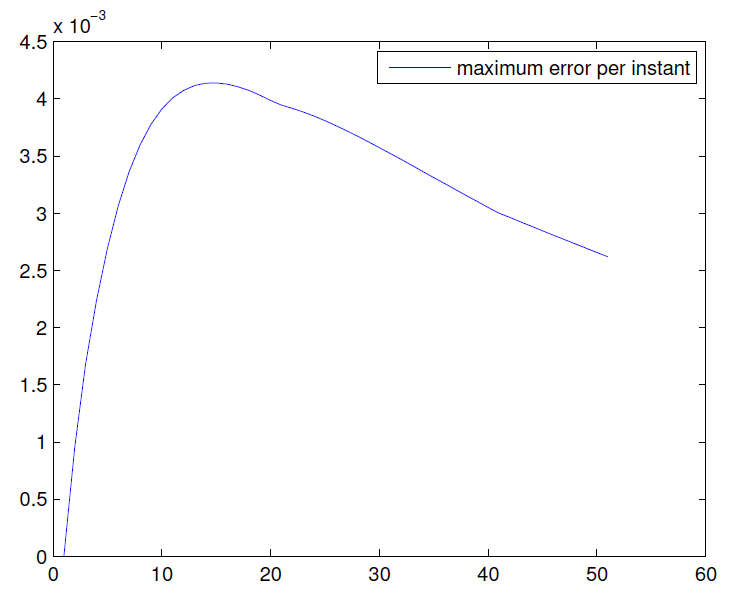
\includegraphics[width=0.45\textwidth]{maxerror.png}}
	\subfloat[$U(x_i,t_j)$, $i,j=1,2,\ldots,51$]{\label{fig7:3}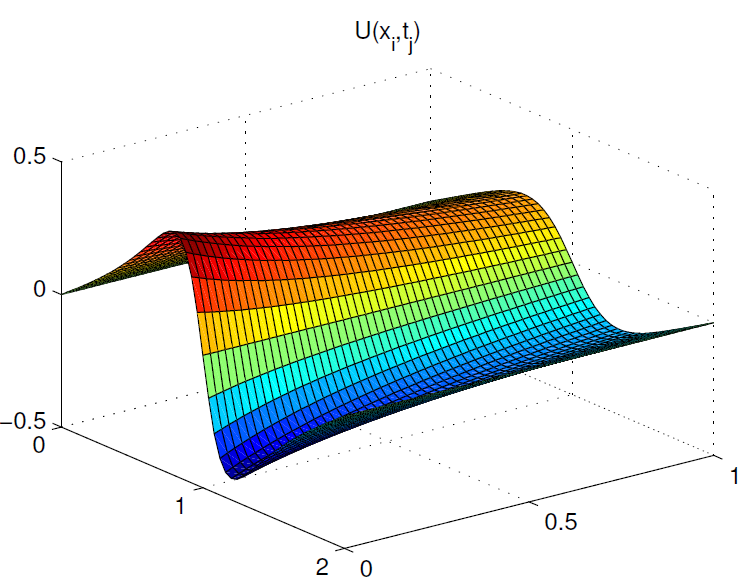
\includegraphics[width=0.45\textwidth]{estimatedU.png}}
	%  \subfloat[$\beta=1$]{\label{fig7:4}\includegraphics[width=0.24\textwidth]{maxerror_beq1_neq50.png}}
	\caption{Error máximo por instante y solución estimada}
	\label{fig:7}
\end{figure}

Es importante destacar que las soluciones estimadas obtenidas han sido comparadas con la exacta (cuyo procedimiento de obtención es detallado en la Sección \ref{uanalitica}), hasta el decimoquinto decimal, para cada uno de los nodos, mostrando que todos los métodos aplicados consiguen el mismo error máximo exacto $MEE=0.004140236998958$ (Maximum Exact Error, por sus siglas en inglés) por cada columna de la matriz solución $U$, es decir la misma diferencia máxima entre la solución exacta y la obtenida iterativamente en cada instante (ver Figura \ref{fig:7}); lo cual es razonable siendo que todos los miembros usados tienen el mismo orden y que el error del proceso de discretización es de orden dos. De la Tabla \ref{tabla1}, deducimos que, en términos de precisión de la solución estimada, los miembros de la familia de métodos iterativos cuyos valores del parámetro son próximos a cero, son más precisos, lo cual concuerda con los resultados del análisis dinámico realizado en \cite{napoles}. El orden de convergencia computacional aproximado $\rho$ también está alrededor de los valores esperados.	

\section{Nueva familia de métodos de orden tres}\label{seccionHGsistemas}
En esta sección presentamos la extensión a sistemas de la familia de Homeier generalizado introducida en la Sección \ref{seccionHG}. Así pues, dicha familia también puede ser utilizada para resolver sistemas de ecuaciones no lineales del tipo $F(x)=0$. Su expresión iterativa es
\begin{equation} \label{schemehgsis}
	\begin{array} {rcl}
		y^{(k)}  & = & x^{(k)}- \varphi F'(x^{(k)})^{-1} F(x^{(k)}), \\
		x^{(k+1)}& = & x^{(k)}-\left[ \gamma F'(y^{(k)})^{-1} F(x^{(k)})+ \delta F'(x^{(k)})^{-1} F(x^{(k)}) \right],
	\end{array}
\end{equation}
donde $\varphi$, $\gamma$ y $\delta$ son parámetros reales.

El resto del capítulo está organizado de la siguiente forma: en la Sección \ref{ordenhgsistemas} se analiza el orden de convergencia de la familia (\ref{schemehgsis}). Posteriormente, en la Sección \ref{numericabratu} se estudia el problema unidimensional de Bratu, obteniendo los resultados de distintos miembros de la familia y comparándolos con los de algunos métodos ya conocidos. Finalmente se presentan algunos comentarios y conclusiones.

Cabe destacar que estos resultados han sido publicados por la revista \textit{``SeMA Journal''}, bajo el título \textit{``Multidimensional Homeier’s generalized class and its application to planar 1D Bratu problem''} (véase \cite{paperhomeiersistemas}).

\subsection{Orden de convergencia}\label{ordenhgsistemas}
Como vamos a demostrar a continuación, los métodos de la familia (\ref{schemehgsis}) tienen orden de convergencia tres para una determinada relación entre sus parámetros.

El siguiente resultado describe cuales son esas condiciones bajo las cuales la familia (\ref{schemehgsis}) tiene orden de convergencia tres. En la demostración usamos la notación y las herramientas presentadas en la Sección \ref{taylorconceptosprevios} del Capítulo \ref{capituloconceptosprevios} (véase también \cite{CHMT}, para más información).

\begin{theorem} \label{t1}
	Sea $\alpha \in  D$ el cero de una función suficientemente diferenciable $F : D \subseteq \mathbb{R}^n \to \mathbb{R}^n$ en un conjunto abierto convexo $D$ con una matriz Jacobiana $F'(x)$ no singular en $\alpha$. Si $\varphi=\frac{1}{2\gamma}$ y $\delta=1-\gamma$, entonces los métodos de la familia (\ref{schemehgsis}) tienen orden de convergencia tres, y su ecuación del error está dada por
	\begin{equation*}
	e^{(k+1)} = \left[ \left( -3+8\gamma-4\gamma^2 \right)C_2^2+\left( \frac{11}{4}-6\gamma+3\gamma^2\right)C_3 \right] {e^{(k)}}^3+O({e^{(k)}}^4),
	\end{equation*}
	donde $C_k=\dfrac{1}{k!}[F'(\alpha)]^{-1}F^{(k)}(\alpha)$,   $k=2,3, \ldots$  y $e^{(k)}=x^{(k)}-\alpha$.
\end{theorem}
\begin{proof}
	Si usamos el desarrollo en series de Taylor de $F\left(x^{(k)}\right)$ y $F'\left(x^{(k)}\right)$ alrededor de $\alpha$, obtenemos	
	\begin{equation*} \label{tay1}
	F\left( x^{(k)} \right)=F'(\alpha)\left\{ e^{(k)}+C_2{e^{(k)}}^2+C_3{e^{(k)}}^3 \right\}+O({e^{(k)}}^4)
	\end{equation*}
	y
	\begin{equation}\label{tay2}
	F'\left( x^{(k)} \right)=F'(\alpha)\left\{ I+2C_2e^{(k)}+3C_3{e^{(k)}}^2 \right\}+O({e^{(k)}}^3).
	\end{equation}
	De  (\ref{tay2}), calculamos la expresión de la inversa
	\begin{equation} \label{tay3}
	\left[ F'\left(x^{(k)}\right)\right]^{-1}=\left\{I+X_2e^{(k)}+X_3{e^{(k)}}^2 \right\}\left[F'(\alpha)\right]^{-1}+O({e^{(k)}}^3),
	\end{equation}
	donde $X_2=-2C_2$, $X_3=4C_2^2-3C_3$ e $I$ denota la matriz identidad de tamaño $n \times n$.\\
	Estos valores han sido obtenidos imponiendo las siguientes condiciones,
	\[
	\left[ 	F'\left(x^{(k)}\right) \right]^{-1}F'\left(x^{(k)}\right)=F'\left(x^{(k)}\right)\left[
	F'\left(x^{(k)}\right)   \right]^{-1}=I.
	\]
	
	Así pues, la expresión del error en el primer paso del método es
	\begin{equation*}
	e_y^{(k)}=y^{(k)}-\alpha  = (1-\varphi)e^{(k)}+\varphi C_2e^{(k)^2}+O(e^{(k)^3}).
	\end{equation*}
	Además, sabemos que
	\begin{equation} \label{tayFsistemas}
	F'\left(y^{(k)}\right) = F'(\alpha)\left\{I+2C_2e_y^{(k)}+3C_3e_y^{(k)^2}\right\}+O(e_y^{(k)^3}).
	\end{equation}
	De forma similar a (\ref{tay3}),
	\begin{equation} \label{tay4}
	\left[F'\left(y^{(k)}\right)\right]^{-1}=\left\{I+Y_2e_y^{(k)}+Y_3e_y^{(k)^2}\right\}\left[F'(\alpha)\right]^{-1}+O(e_y^{(k)^3}),
	\end{equation}
	donde $Y_2=-2C_2$ y $Y_3=4C_2^2-3C_3$.
	
	Y, si reemplazamos en (\ref{tay4}) las potencias de $e_y^{(k)}=y^{(k)}-\alpha$, obtenemos, después de realizar algunas operaciones algebraicas
	\begin{align} \label{tay5}
	\left[F'\left(y^{(k)}\right)\right]^{-1} \nonumber = & \left\{I-2(1-\varphi)C_2e^{(k)}+\left[(4-10\varphi+4\varphi^2)C_2^2+(-3+6\varphi+3\varphi^2)C_3\right]e^{(k)^2}\right\}\left[F'(\alpha)\right]^{-1}\\
	& +O(e^{(k)^3}).
	\end{align}
	
	Finalmente, la ecuación del error es expresada como,
	\begin{align} \label{errorgenerico}
	e^{(k+1)} = & (1-\gamma-\delta)e^{(k)}+(\gamma+\delta-2\varphi\gamma)C_2e^{(k)^2}\\\nonumber &+\left[(8\varphi\gamma-2\gamma-2\delta-4\varphi^2\gamma)C_2^2+(2\gamma+2\delta-6\varphi\gamma+3\varphi^2\gamma)C_3\right]e^{(k)^3}+O(e^{(k)^4}).
	\end{align}
	
	Si forzamos que los términos correspondientes a $e^{(k)}$ y $e^{(k)^2}$ sean eliminados en (\ref{errorgenerico}), obtenemos el siguiente sistema:
	\begin{equation*}
	\left. \begin{array} {lcc}
	1- \gamma- \delta            &  = & 0 \\
	\gamma+\delta-2\varphi\gamma  &  = & 0
	\end{array} \right \},
	\end{equation*}
	cuya solución es $\varphi = \dfrac{1}{2\gamma}$ y  $\delta=1-\gamma$. Esta solución es única, aunque depende de un parámetro libre, $\gamma$. Si reemplazamos $\varphi$ y $\delta$ en (\ref{schemehgsis}), obtenemos una familia uniparamétrica de métodos de orden tres, cuya ecuación del error se puede expresar como:
	\begin{equation}\label{error}
	e^{(k+1)} = \left[ \left( -3+8\gamma-4\gamma^2 \right)C_2^2+\left( \frac{11}{4}-6\gamma+3\gamma^2\right)C_3 \right] {e^{(k)}}^3+O({e^{(k)}}^4),
	\end{equation}
	y el teorema queda demostrado. $\Box$
	\vspace{.5cm}
\end{proof}

Denotamos los miembros de la familia obtenida
\begin{equation} \label{HG}
\begin{array} {rcl}
y^{(k)}  & = & x^{(k)}- \dfrac{1}{2 \gamma} F'(x^{(k)})^{-1} F(x^{(k)}), \\
x^{(k+1)}& = & x^{(k)}-\left[ \gamma F'(y^{(k)})^{-1} F(x^{(k)})+ (1-\gamma) F'(x^{(k)})^{-1} F(x^{(k)}) \right],
\end{array}
\end{equation}
por $HG(\gamma)$, algunos de ellos serán usados en la sección de resultados numéricos. Es importante mencionar en cuanto a la ecuación del error (\ref{error}), que algunos de los valores interesantes del parámetro $\gamma$ son las raíces de $-3+8\gamma-4\gamma^2=0$, esas son, $\gamma=1/2$ y $\gamma=3/2$, y las raíces de $\frac{11}{4}-6\gamma+3\gamma^2=0$, $\gamma = (6-\sqrt{3})/6$ y $\gamma = (6+\sqrt{3})/6$. Estos valores reducen el error asintótico. 

\subsection{Estimación numérica de la solución del problema de Bratu}\label{numericabratu}
En esta sección presentamos el problema unidimensional de Bratu \cite{bratu}, lo transformamos en un sistema no lineal aplicando diferencias finitas simétricas de segundo orden y resolvemos dicho sistema usando algunos de los métodos iterativos de la familia (\ref{HG}).

El clásico problema de Bratu es una ecuación en derivadas parciales elíptica no lineal con condiciones de contorno homogéneas tipo Dirichlet. El problema viene dado por
\begin{align} \label{bratu}
\Delta u+Ce^u&=0 \quad \text{en } \Omega, \\ \nonumber
u&=0 \quad \text{en } \delta \Omega,
\end{align}
donde $C >0$ y $\Omega$ es un dominio acotado con límite $\delta \Omega$. Es un problema no lineal comunmente usado como prueba comparativa de resultados entre diferentes métodos numéricos. En el caso unidimensional, el problema se reduce a la expresión
\begin{equation} \label{bratu1d}
\dfrac{d^2u}{dx^2}+Ce^u=0, \quad 0 \leq x \leq 1,
\end{equation}
cuyas condiciones de contorno son
\begin{equation} \label{bratu1dboundary}
u(0)=u(1)=0.
\end{equation}

El problema de Bratu aparece en una gran variedad de áreas y aplicaciones, como el modelo de ignición de combustión térmica de fuel, la transferencia radiada de calor, la reacción termal, el modelo de Chandrasekhar de la expansión del universo, la teoría de los reactores químicos (véase \cite{bratu2,bratu4,bratu5,bratu3}). En \cite{bratu4} se encuentra un resumen histórico del problema.

El problema de Bratu contiene un parámetro $C$ y tiene dos soluciones para $C < C_c$ que nos llevan siempre a la obtención de dos ramas, llamadas rama inferior y superior. En caso de que $C=C_c$ (donde $C_c=3.513830719$), sólo existe una única solución, y si $C>C_c$ no existe ninguna. La recta del término de la derecha de la ecuación \eqref{cosh} es tangente al $cosh(\alpha)$ para $C=C_c$, y de ahí que sea el valor crítico.

La solución exacta del problema unidimensional de Bratu descrito en (\ref{bratu1d}) y (\ref{bratu1dboundary}), está dada por:

\begin{equation}\label{exact}
u(x)=2\ln{\left[\frac{\cosh{(\alpha)}}{\cosh{(\alpha(1-2x))}}\right]},
\end{equation}
donde $\alpha$ satisface la ecuación trascendente
\begin{equation}\label{cosh}
\cosh{(\alpha)}=\frac{4}{\sqrt{2C}} \alpha.
\end{equation}

La solución de esta ecuación no lineal puede ser obtenida mediante el uso de algún método iterativo, como por ejemplo el de Newton, cuyos resultados se pueden observar en la Tabla \ref{alphas}, para tres valores de $C$, tales como $C=0.1$, $C=1.0$ y $C=3.0$.
Nótese que dependiendo de la estimación inicial del método iterativo se obtiene el valor correspondiente a la rama inferior o a la superior.

\begin{table}[h!]\centering
	\begin{tabular}{c|c|c|}
		\cline{2-3}
		\multicolumn{1}{l|}{}       & \multicolumn{2}{c|}{Valor de $\alpha$} \\ \hline
		\multicolumn{1}{|c|}{$C$}   & Rama inferior     & Rama superior     \\ \hline
		\multicolumn{1}{|c|}{0.1}   & 0.1125               & 4.3554               \\ \hline
		\multicolumn{1}{|c|}{1.0}   & 0.3793               & 2.7347               \\ \hline
		\multicolumn{1}{|c|}{3.0}   & 0.8434               & 1.6441               \\ \hline
	\end{tabular}
	\caption{Ambas soluciones de la ecuación presentada en (\ref{cosh}), para distintos valores de $C$.}\label{alphas}
\end{table}

La solución del problema de Bratu usando diferencias finitas, implica la discretización de la ecuación diferencial (\ref{bratu1d}), incluyendo las condiciones de contorno (\ref{bratu1dboundary}).
El método transforma el problema en un sistema de ecuaciones no lineales simultáneas, el cual es resuelto mediante el uso de de distintos métodos iterativos: Newton ($N$), Traub ($T$) (véase \cite{TR}), y algunos de los miembros de la familia $HG(\gamma)$. Usando un mallado uniforme con paso  $h=1/(n+1)$, para un entero positivo $n$, el rango $0 \leq x \leq 1$ es discretizado como $x_j=0+jh$, con $j=0,1, \ldots,n+1$. Usando un esquema en diferencias finitas simétricas y estándar (DFE), la versión discretizada del problema de Bratu será
\begin{equation} \label{sfd}
\frac{u_{i+1}-2u_i+u_{i-1}}{hs}+Ce^{u_i}=0,  \quad i=1,2 \ldots, n,
\end{equation}
donde $hs=h^2$, con $u_0=u_{n+1}=0$.

Por otro lado, un esquema en diferencias finitas no estándar (DFNE) de Mickens \cite{buckmire}, también puede ser usado, el cual produce
\begin{equation}\label{nsfd}
\frac{u_{i+1}-2u_i+u_{i-1}}{hs}+Ce^{u_i}=0, \quad i=1,2, \ldots,n,
\end{equation}
donde $hs=2\ln{[\cosh{(h)}]}$. En el límite cuando $h$ tiende a cero, el esquema DFNE se reduce al DFE.

Resultados previos dados por Buckmire en \cite{buckmire} muestran que el error debido a las diferencias finitas decrece proporcionalmente a $h^2$.
También, los errores del DFNE son consistentemente más pequeños que los del DFE, como se puede observar en las Tablas \ref{tsfd} y \ref{tnsfd}.

Para tratar el sistema no lineal resultante, es bien conocido que la solución es mucho más fiable y se obtiene mucho más deprisa si la aproximación inicial está cerca de la solución. En consecuencia, para resolver iterativamente el sistema no lineal resultante, utilizamos como estimación inicial una simple función sinusoidal (similar a la usada por Boyd \cite{boyd}) con una amplitud apropiada $a$ (la cual satisface las condiciones de cotorno). Concretamente, para la rama inferior, $a$ se debería coger como $a < u_c$, mientras que la rama superior requiere $a>u_c$ (de lo contrario podría suceder que debido a una aproximación inicial mala, nuestro método convergiera a la solución opuesta), donde $u_c$ es la solución única de (\ref{exact}) cuando $C=C_c$. En nuestro caso hemos decidido tomar $a=1$ y $a=8$, respectivamente, como fue sugerido en \cite{mohsen}, siendo la función sinusoidal inicial
\begin{equation}
s(x)=a \sin(\pi x).
\end{equation}

Hemos aplicado los tres métodos $N$, $T$ y  $HG(\gamma)$ para los tres valores de $C$ que también fueron usados en la Tabla \ref{alphas}, cogiendo $n=20$ y un criterio de parada tal que $\|x^{(k+1)}-x^{(k)} \|+\|F(x^{(k)} \|< 10^{-10}$ para todos los casos (reducir la tolerancia no incrementaría la precisión de la solución, ya que estamos condicionados por el proceso de discretización). Una comparativa entre el error máximo (máxima diferencia entre la solución exacta obtenida de (\ref{exact}) y la estimada por el método iterativo) para cada valor de $C$, así como para ambas ramas inferior y superior, es mostrada en las Tablas \ref{tsfd} y \ref{tnsfd}, para DFE y DFNE, respectivamente. La solución estimada, computacionalmente obtenida mediante los tres métodos, sólo difiere a partir del decimosexto decimal, por lo que los resultados mostrados en esas tablas son los mismos para todos ellos. De hecho, en el caso específico de $HG(\gamma)$, cuatro miembros de la familia son puestos a prueba, $\gamma=1/2$, $\gamma=3/2$, $\gamma=(6-\sqrt{3})/6$ y $\gamma=(6+\sqrt{3})/6$; aquellos correspondientes a los valores del parámetro que reducen el error asintótico y que además están en la zona estable del plano de parámetros obtenido en el Capítulo \ref{capitulodinamica}. La misma solución estimada ha sido obtenida para los cuatro, luego los resultados mostrados en las Tablas \ref{tsfd} y \ref{tnsfd} son idénticos para los cuatro valores cogidos del parámetro $\gamma$.

\begin{table}[h!]
	\parbox{.45\linewidth}{
		\centering
		\begin{tabular}{c|c|c|}
			\cline{2-3}
			\multicolumn{1}{l|}{}       & \multicolumn{2}{c|}{Error máximo} \\ \hline
			\multicolumn{1}{|c|}{$C$}   & Rama inferior     & Rama superior     \\ \hline
			\multicolumn{1}{|c|}{0.1}   & 2.8802e-6        & 0.0185   \\ \hline
			\multicolumn{1}{|c|}{1.0}   & 2.5816e-5        & 0.0062    \\ \hline
			\multicolumn{1}{|c|}{3.0}   & 0.0010           & 0.0040    \\ \hline
		\end{tabular}
		\caption{Error máximo obtenido aplicando DFE.}\label{tsfd}
	}
	\hfill
	\parbox{.45\linewidth}{
		\centering
		\begin{tabular}{c|c|c|}
			\cline{2-3}
			\multicolumn{1}{l|}{}       & \multicolumn{2}{c|}{Error máximo} \\ \hline
			\multicolumn{1}{|c|}{$C$}   & Rama inferior     & Rama superior     \\ \hline
			\multicolumn{1}{|c|}{0.1}   & 1.9310e-6        & 0.0182   \\ \hline
			\multicolumn{1}{|c|}{1.0}   & 3.4198e-5        & 0.0058  \\ \hline
			\multicolumn{1}{|c|}{3.0}   & 5.2045e-4        & 0.0030   \\ \hline
		\end{tabular}
		\caption{Error máximo obtenido aplicando DFNE.}\label{tnsfd}
	}
\end{table}

Los resultados muestran una buena precisión para todos los valores de $C$, con una menor exactitud para la rama superior.
También es interesante observar el distinto comportamiento que ambas ramas, inferior y superior, tienen en cuanto al vector de errores absolutos (el vector que contiene la diferencia entre la solución exacta y la estimada para cada valor de $x$). En las Figuras \ref{flower} y \ref{fupper} podemos ver que mientras que en el caso de la rama inferior, el error máximo está situado en el medio ($x=1/2$), para el caso de la rama superior hay dos máximos localizados en ambos lados de este. Ambas figuras han sido obtenidas aplicando $HG(\gamma)$, con $\gamma=1/2$, $C=1$, $n=20$
y una tolerancia de $10^{-10}$.

\begin{figure}[h!]\centering
	\begin{minipage}[m]{0.38\linewidth}
		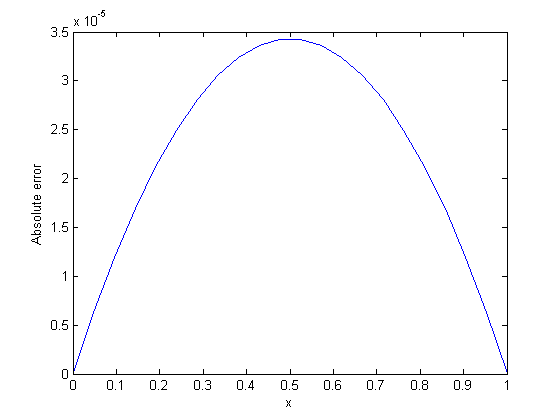
\includegraphics[width=1.1\textwidth]{figure_lower.png}
		\caption{Error absoluto de la rama inferior. HG(1/2), $C=1$ y $n=20$.}
		\label{flower}
	\end{minipage}\hspace{2cm}
	\begin{minipage}[m]{0.38\linewidth}
		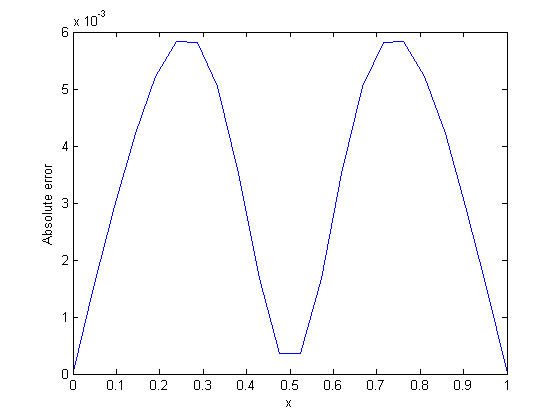
\includegraphics[width=1.1\textwidth]{figure_upper.png}
		\caption{Error absoluto de la rama superior. HG(1/2), $C=1$ y $n=20$.}
		\label{fupper}
	\end{minipage}	
\end{figure}

Aunque no existe prácticamente ninguna diferencia entre la solución estimada de los tres métodos estudiados, sí hay una diferencia en la cantidad de iteraciones de las que requiere cada método para alcanzar la solución estimada. En las Tablas de la \ref{iter1} a la \ref{iter4}, se muestra, para los cuatro miembros mencionados de la familia $HG(\gamma)$ que minimizan el error asintótico, y para distintos valores de $C$ y de las ramas inferior y superior (RI y RS, respectivamente), el número de iteraciones requeridas para nuestro método $HG(\gamma)$ comparado con el clásico método de Newton y de Traub. Nótese que todos los miembros probados de la familia no sólo convergen siempre más rápidamente que el método de Newton, sino también que el de Traub, en algunos casos. En cuando a cantidad de iteraciones requeridas, no hay ninguna diferencia entre usar DFE y DFNE, ya que DFNE incrementa la precisión de la discretización, pero no afecta la del método iterativo.

\begin{figure}[h!]
	\subfloat[$HG(1/2)$]{\parbox{.45\linewidth}{
			\centering
			\begin{tabular}{c|c|c|c|c|c|c|}
				\cline{2-7}
				& \multicolumn{6}{c|}{No. de iter. $\gamma=1/2$}         \\ \hline
				\multicolumn{1}{|c|}{\multirow{2}{*}{C}} & \multicolumn{3}{c|}{RI} & \multicolumn{3}{c|}{RS} \\ \cline{2-7}
				\multicolumn{1}{|c|}{}                   & N      & T     & HG    & N      & T     & HG     \\ \hline
				\multicolumn{1}{|c|}{0.1}                & 2      & 1     &  1     & 5      & 3     & 3       \\ \hline
				\multicolumn{1}{|c|}{1.0}                & 3      & 2     & 2      & 8      &  5    & 4       \\ \hline
				\multicolumn{1}{|c|}{3.0}                & 4      & 3     & 2      &  6     & 4     &  3      \\ \hline
			\end{tabular}
		}\label{iter1}}
	\hfill
	\subfloat[$HG(3/2)$]{\parbox{.45\linewidth}{
			\centering
			\begin{tabular}{c|c|c|c|c|c|c|}
				\cline{2-7}
				& \multicolumn{6}{c|}{No. de iter. $\gamma=3/2$}         \\ \hline
				\multicolumn{1}{|c|}{\multirow{2}{*}{C}} & \multicolumn{3}{c|}{RI} & \multicolumn{3}{c|}{RS} \\ \cline{2-7}
				\multicolumn{1}{|c|}{}                   & N       & T     & HG & N       & T      & HG     \\ \hline
				\multicolumn{1}{|c|}{0.1}                & 2       & 1     &  1      &  5      &  3     & 3       \\ \hline
				\multicolumn{1}{|c|}{1}                  & 3       &  2    &  2      &  8      & 5      & 5       \\ \hline
				\multicolumn{1}{|c|}{3}                  & 4       &  3    & 2       & 6       & 4      &  4      \\ \hline
			\end{tabular}
		}\label{iter2}}
	\\
	\subfloat[$HG((6-\sqrt{3})/6)$]{\parbox{.45\linewidth}{
			\centering
			\begin{tabular}{c|c|c|c|c|c|c|}
				\cline{2-7}
				& \multicolumn{6}{c|}{No. de iter. $\gamma=(6-\sqrt{3})/6$}         \\ \hline
				\multicolumn{1}{|c|}{\multirow{2}{*}{C}} & \multicolumn{3}{c|}{RI} & \multicolumn{3}{c|}{RS} \\ \cline{2-7}
				\multicolumn{1}{|c|}{}                   & N      & T     & HG     & N      & T     & HG     \\ \hline
				\multicolumn{1}{|c|}{0.1}                & 2      & 1     &  1     & 5      & 3     & 3       \\ \hline
				\multicolumn{1}{|c|}{1}                  &  3     & 2     &  1     &  8     &  5    &  4      \\ \hline
				\multicolumn{1}{|c|}{3}                  &  4     & 3     &  2     &  6     &   4   &  4      \\ \hline
			\end{tabular}
		}\label{iter3}}
	\hfill
	\subfloat[$HG((6+\sqrt{3})/6)$]{\parbox{.45\linewidth}{
			\centering
			\begin{tabular}{c|c|c|c|c|c|c|}
				\cline{2-7}
				& \multicolumn{6}{c|}{No. de iter. $\gamma=(6+\sqrt{3})/6$}         \\ \hline
				\multicolumn{1}{|c|}{\multirow{2}{*}{C}} & \multicolumn{3}{c|}{RI} & \multicolumn{3}{c|}{RS} \\ \cline{2-7}
				\multicolumn{1}{|c|}{}                   & N      & T     & HG     & N      & T     & HG     \\ \hline
				\multicolumn{1}{|c|}{0.1}                & 2      &  1    &  1     & 5      & 3     &  3      \\ \hline
				\multicolumn{1}{|c|}{1}                  & 3      & 2     & 2      &  8     &  5    & 5       \\ \hline
				\multicolumn{1}{|c|}{3}                  & 4      &  3    &  2     &  6     & 4     & 4       \\ \hline
			\end{tabular}
		}\label{iter4}}
	\caption{Número de iteraciones para diferentes valores de $\gamma$.}
\end{figure}